\documentclass{article}
\iffalse
This file is protected by Copyright. Please refer to the COPYRIGHT file
distributed with this source distribution.

This file is part of OpenCPI <http://www.opencpi.org>

OpenCPI is free software: you can redistribute it and/or modify it under the
terms of the GNU Lesser General Public License as published by the Free Software
Foundation, either version 3 of the License, or (at your option) any later
version.

OpenCPI is distributed in the hope that it will be useful, but WITHOUT ANY
WARRANTY; without even the implied warranty of MERCHANTABILITY or FITNESS FOR A
PARTICULAR PURPOSE. See the GNU Lesser General Public License for more details.

You should have received a copy of the GNU Lesser General Public License along
with this program. If not, see <http://www.gnu.org/licenses/>.
\fi

% TODO: Version numbers?
\usepackage{graphicx}
\graphicspath{ {figures/} }
\usepackage{fancyhdr}
\usepackage{colortbl}
\usepackage[margin=.75in]{geometry}
\usepackage[justification=centering]{caption}
\pagestyle{fancy}
\lhead{Zipper/Myriad-RF 1 Daughtercards}
\rhead{ANGRYVIPER Team}
\definecolor{drkgreen}{rgb}{0,.6,0}
\renewcommand{\headrulewidth}{0pt}
\definecolor{blue}{rgb}{.7,.8,.9}
\begin{document}
\textbf{Important Note: The Zipper Carrier Card is no longer being produced by the manufacturer. The card is Open Source so you are able to fabricate one yourself.}
\section*{Required Modifications for Myriad-RF 1 and Zipper Daughtercards}
To support OpenCPI RF applications on the Zedboard (zed), Xilinx Virtex6 (ml605), and Altera Stratix 4 (alst4) development kits, 2 daughtercards are required:\par
	\begin{itemize}
	\item[1)] Myriad-RF 1 board
	\item[2)] Zipper FMC/HSMC carrier card for Myriad-RF 1
	\end{itemize}
	\begin{figure}[ht]
	\centering
		\begin{minipage}{.5\textwidth}
			\centering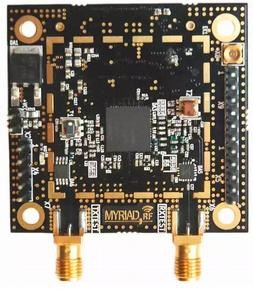
\includegraphics[width=0.65\linewidth]{myriadrf}
			\captionof{figure}{Myriad-RF 1 Board}
			\label{fig:myriadrf}
		\end{minipage}%
		\begin{minipage}{.5\textwidth}
			\centering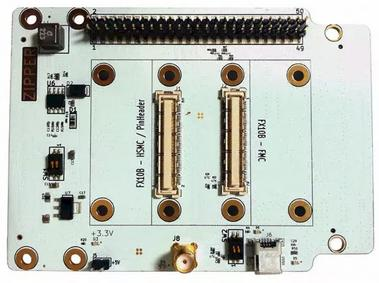
\includegraphics[width=1.0\linewidth]{zipper}
			\captionof{figure}{Zipper FMC/HSMC carrier card for Myriad-RF 1}
			\label{fig:zipper}
		\end{minipage}
	\end{figure}
\noindent The Myriad-RF 1 is a transmit/receive digital-to-RF module based on the Lime Microsystems LMS6002D transceiver IC. The Zipper carrier card provides an adapter for the Myriad-RF 1 ADC/DAC interface to both FMC and HSMC connectors. Both daughtercards are commercially available from DigiKey. For additional information on the daughtercards as of October 2016, see the Reference Documentation section of this document and Table~\ref{tab:version_info}.

\section*{Purpose of this Document}
Before using the daughtercards with OpenCPI on the zed, ml605 and alst4 platforms, a number of hardware modifications are required. The below sections describe the modifications in detail for Version 1 Revision 1 (v1 r1) of Myriad-RF 1 and Version 2 Revision 1 or 3 (v2 r1 or v2 r3) of the Zipper carrier card. The schematic for any other revision should be verified prior to making these changes.
		\begin{table}[h]
			\scriptsize
			\begin{center}
  				\begin{tabular}{|c|c|c|c|c|}
    			\hline
    			\rowcolor{blue}
    			Daughtercard & Version & Revision & Digikey Part Number & Price\\
    			\hline
    			Myriad-RF 1 & 1 & 1 & 1434-1001-ND & \$299\\
    			\hline
    			Zipper Carrier Card & 2 & 1 or 3 & 1434-1002-ND & \$199\\
    			\hline
   				\end{tabular}
   				\captionof{table}{Daughtercard Version \& Part Numbers}
   				\label{tab:version_info}
		  	\end{center}
   		\end{table}
\pagebreak

\normalsize
\subsection*{Zipper: Known Issues}
The HSMC and FMC slot specifications include card presence pins which allow an FPGA host board to determine the presence of an HSMC/FMC mezzanine card via the mezzanine card shorting these pins to ground. Note that the Zipper Board v.2 r.1 does not short the FMC H2 PRSNT\_M2C\_L pin to ground. This has the side effect of OpenCPI assemblies erroneously reporting their slotCardIsPresent properties as false for the zed and ml605 platform workers even when a card is present.\par\medskip
\subsection*{Zipper: Configure SW1 for power up}
On the Zipper, SW1 is a manual slider switch that powers on to the Zipper and Myriad cards when power is applied to the Zedboard.  Configuring SW1 for 'always on', allows the Zedboard power switch to act as the system power switch.\par\medskip
\noindent Configure slider switch 1 of SW1 to be in the 'ON' position, as shown in Figure \ref{fig:zipper_sw1_configured}. Note: slider switch 2 is not connected in the schematic.\par\medskip
\noindent Once the system is powered on, two green LEDs (Zipper(D3) and Myriad(LD1)) will illuminate.\par\smallskip
	\begin{figure}[ht]
		\begin{center}
		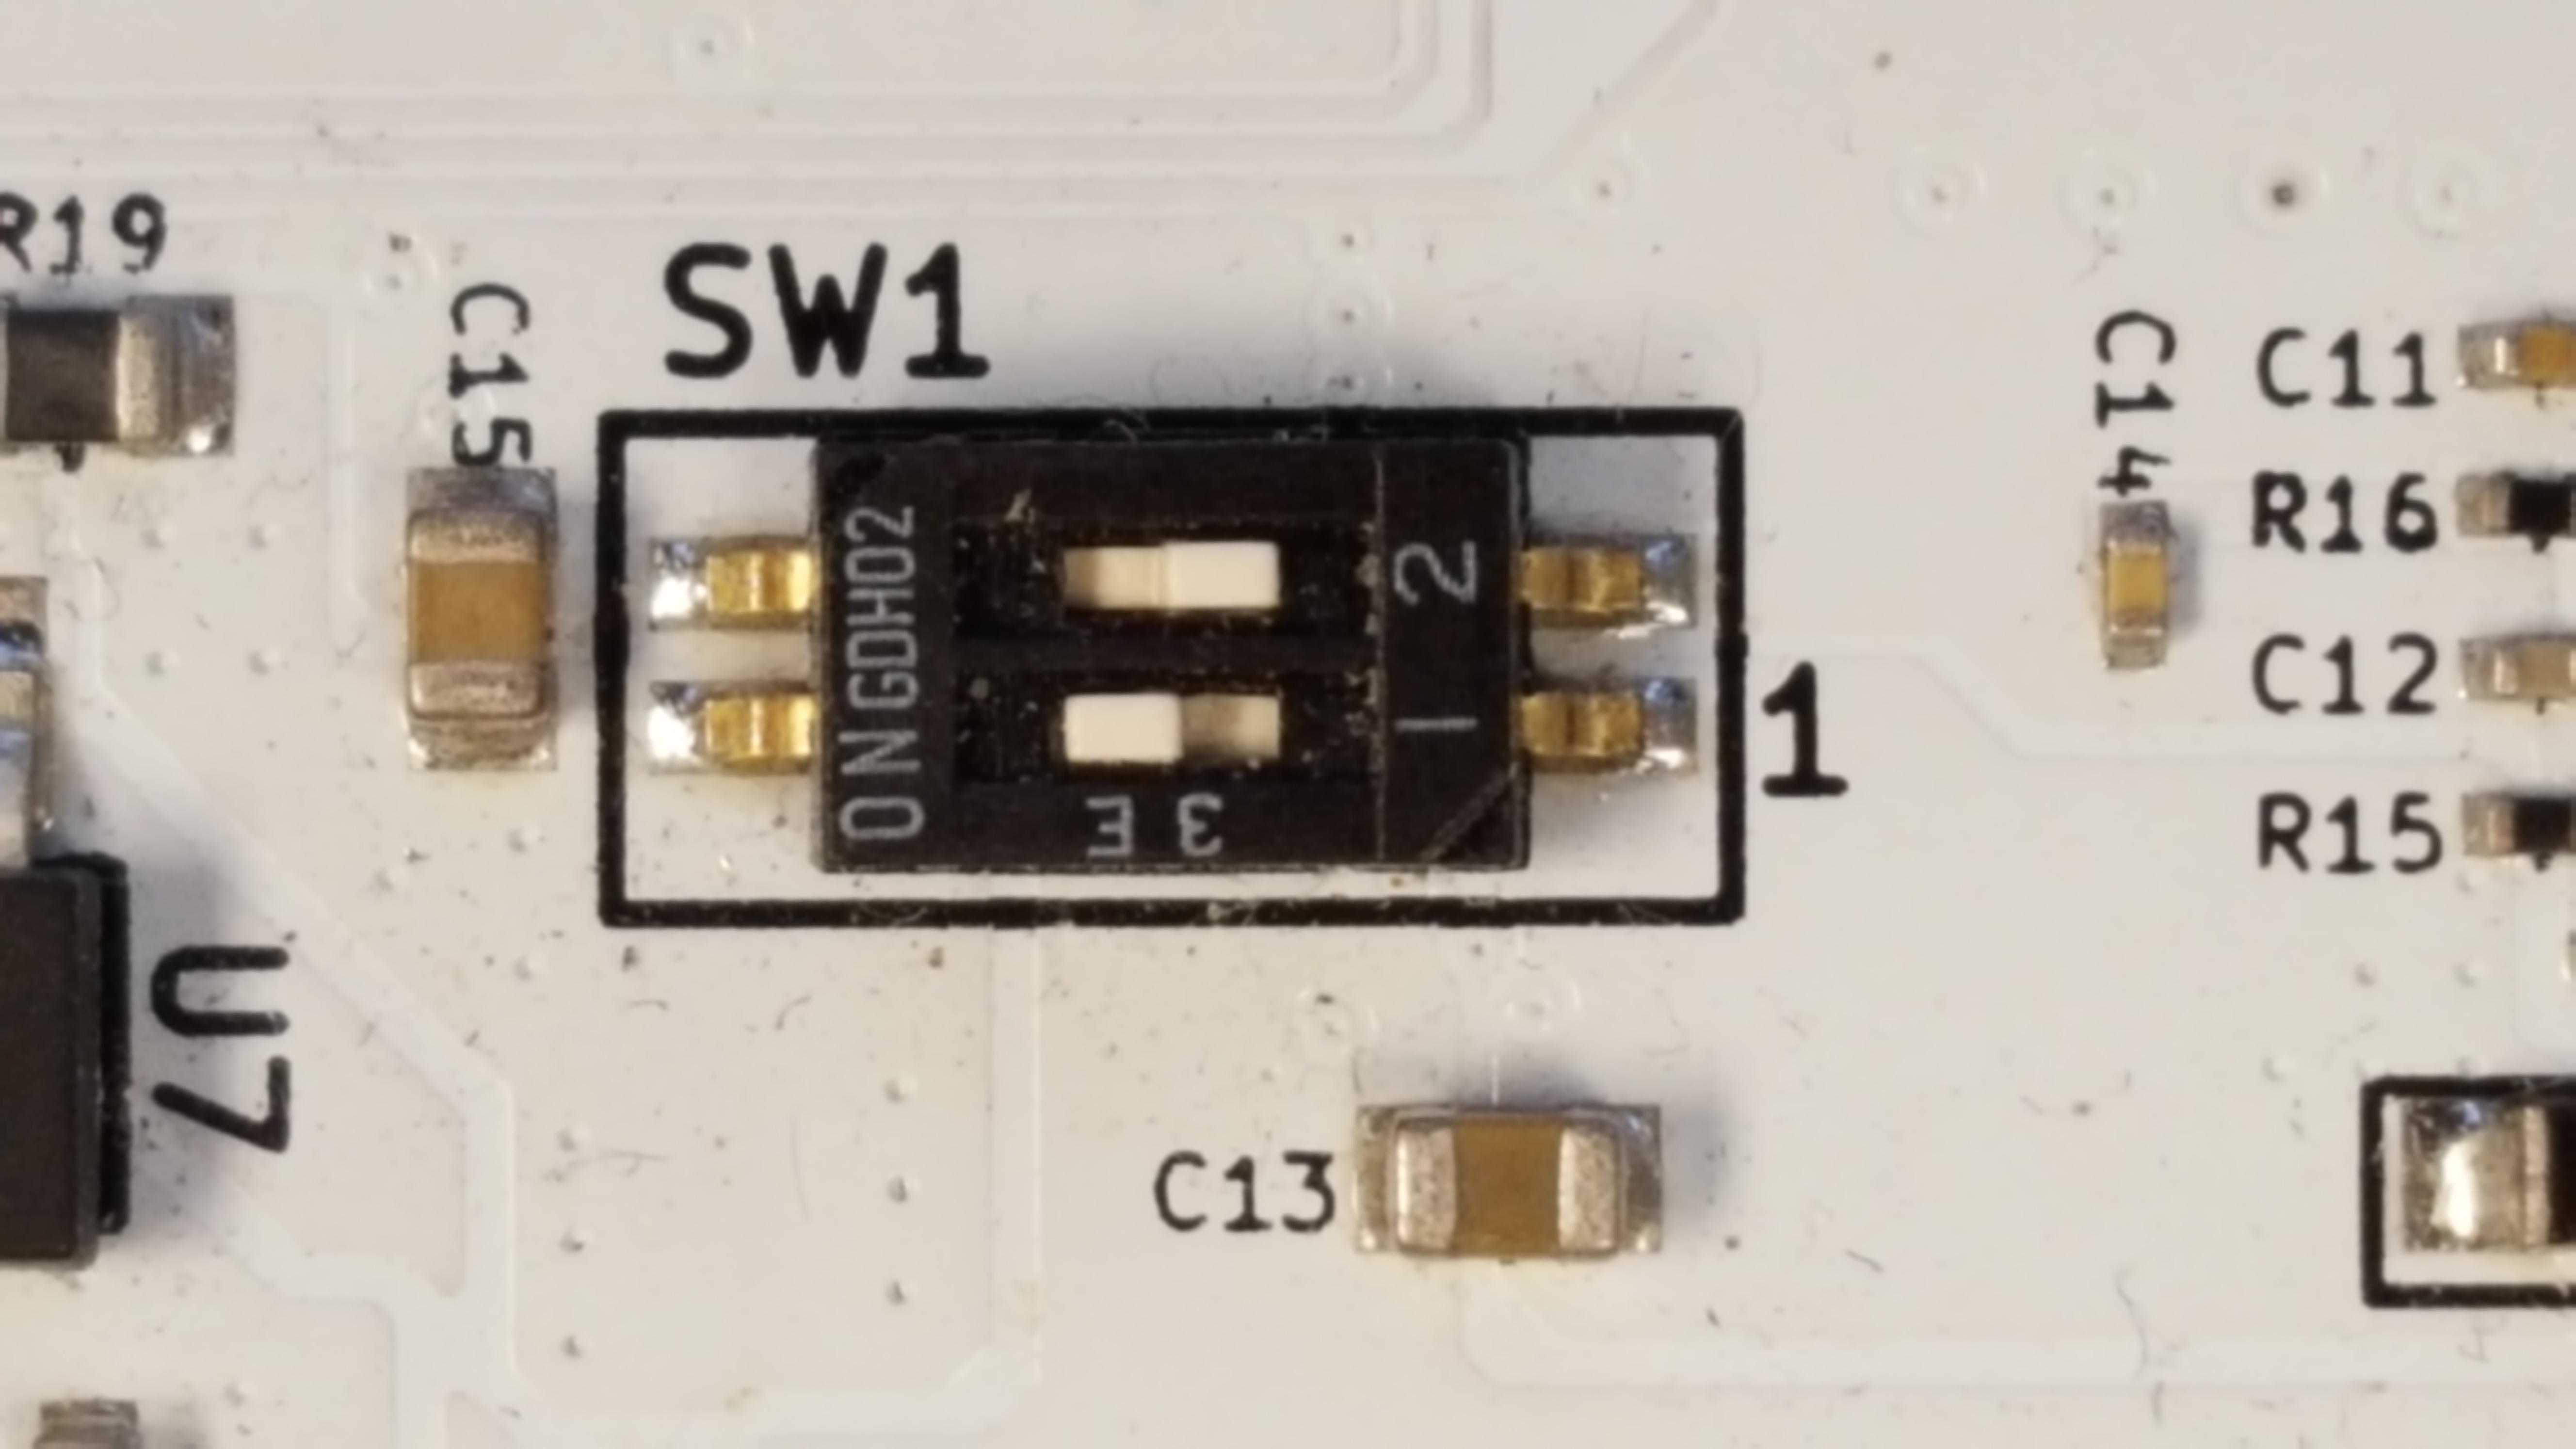
\includegraphics[scale=0.05]{zipper_sw1_configured}
		\caption{Configured Zipper SW1: slider switch 1 is 'ON'}
		\label{fig:zipper_sw1_configured}
		\end{center}
	\end{figure}
\pagebreak

\normalsize
\subsection*{Zipper: Modify voltage divider to set FMC/HSMC IO voltage to 2.5 V}
The input-output (IO) voltage on the Zipper carrier card FMC and HSMC connectors is configurable. A study of the supported OpenCPI platforms was conducted to determine if there was a common I/O voltage that could be used for the FMC/HSMC interfaces. Table \ref{table:io_voltages} lists the supported IO voltages of the OpenCPI platforms. Given this information, 2.5 V is the logical choice because all the platforms support this IO voltage.\par\smallskip
		\begin{table}[h]
			\begin{center}
				\scriptsize
  				\begin{tabular}{|c|c|c|c|}
    			\hline
    			\rowcolor{blue}
    			Platform & Connector Type & Supported IO Voltages\\
    			\hline
    			zed & FMC & 1.8 V, 2.5 V, 3.3 V\\
    			\hline
    			ml605 & FMC & 2.5 V\\
    			\hline
    			alst4 & HSMC & 2.5 V\\
    			\hline
   				\end{tabular}
   				\captionof{table}{OpenCPI Platform IO Voltages}
				\label{table:io_voltages}
		  	\end{center}
   		\end{table}
\normalsize
\noindent On the Zipper carrier card, the IO voltage is determined via a voltage divider circuit, and can be adjusted by replacing one resistor. The default IO voltage is 3.3 V. Figure \ref{fig:zipper_voltage_divider} shows the voltage divider circuit from page 6 of the Zipper schematic \cite{zipper_sch}. To set the IO voltage to 2.5 V, replace R82 with a resistor of value 150 ohms.\par\smallskip
	\begin{figure}[ht]
		\begin{center}
		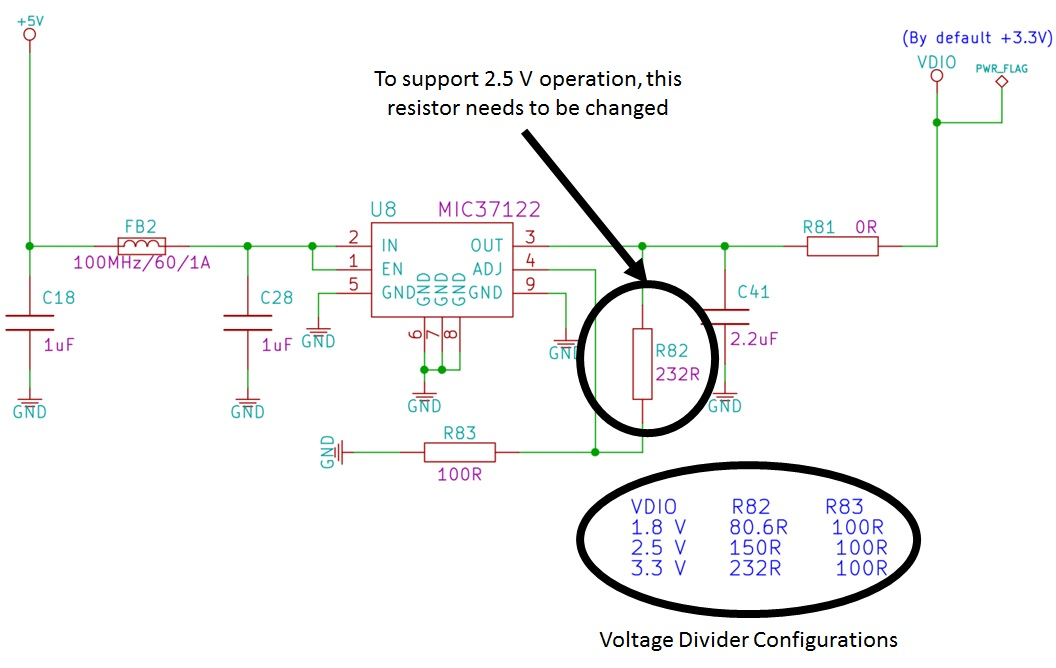
\includegraphics[scale=0.4]{zipper_voltage_divider}
		\caption{Zipper IO Voltage Divider Circuit}
		\label{fig:zipper_voltage_divider}
		\end{center}
	\end{figure}
	\begin{figure}[ht]
		\begin{center}
		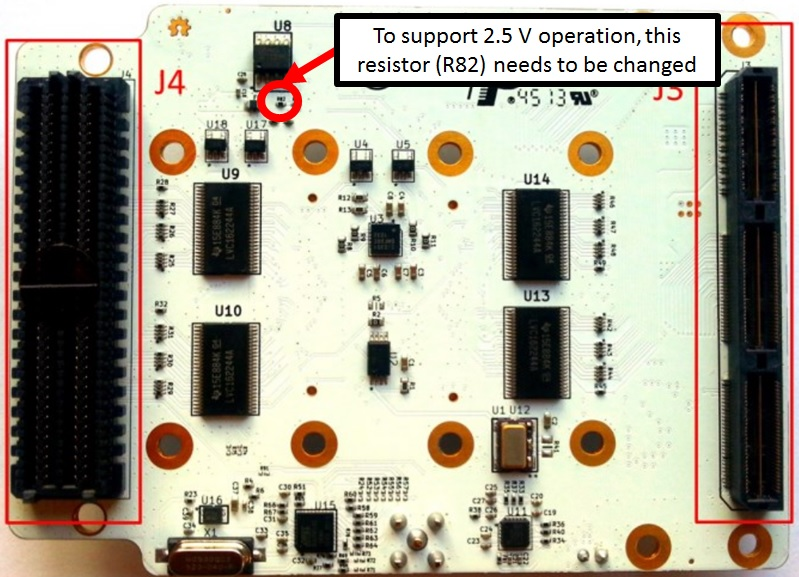
\includegraphics[scale=0.35]{zipper_layout}
		\caption{Zipper IO Voltage Divider Layout}
		\label{fig:zipper_layout}
		\end{center}
	\end{figure}
\pagebreak

\subsection*{Zipper: Connect I2C, SPI, and GPIO buses to FMC/HSMC connectors}
\small
The default mode of operation for control of the Zipper and Myriad-RF 1 is via USB (J6) on the Zipper carrier card. The USB port connects to a microcontroller (U15)  which implements the I2C, SPI, and GPIO buses.\par\medskip
\noindent The OpenCPI mode of operation controls the Zipper and Myriad-RF 1 through HDL device workers on the FPGA and RCC proxy workers, all of which are located on the OpenCPI enabled platform. Therefore, hardware modifications are made to the Zipper to reroute the I2C, SPI and GPIO signals from the microcontroller to the FMC/HSMC connectors which interface to the FPGA. Note: The Zipper has a PLL Frequency Synthesizer (ADF4002) which is currently not supported by AV and these modifications do not support access to the SPI interface of this device.\par\medskip
\noindent The layout of the Zipper carrier card has traces for both USB and FMC/HSMC control with 0 ohm resistors that can be placed or removed depending on which interface is being used. Figures \ref{fig:zipper_microcontroller} and Figures \ref{fig:zipper_layout2} and Table \ref{table:resistors_to_replace} specify which resistors need to be removed and which ones need to be placed to use the Zipper carrier card on OpenCPI platforms.\par\bigskip
	\scriptsize
	\begin{table}[h]
	\begin{center}
	\scriptsize
	\begin{tabular}{|c|c|c|}
		\hline
    	\rowcolor{blue}
    	Description & Resistor to remove & Resistor to place\\
    	\rowcolor{blue}
    	~ & (default is placed) & (default is removed) \\
    	\hline
    	I2C SDA & R76 & R74 \\
    	\hline
    	I2C SCL & R77 & R75 \\
    	\hline
    	SPI RESET & R60 & R24 \\
    	\hline
    	SPI MISO & R61 & R54 \\
    	\hline
    	SPI MOSI & R62 & R55 \\
    	\hline
    	SPI CLK & R63 & R56 \\
    	\hline
    	SPI CS & R64 & R57 \\
    	\hline
    	GPIO0 & R68 & R71 \\
    	\hline
    	GPIO1 & R69 & R72 \\
    	\hline
    	GPIO2 & R70 & R73 \\
    	\hline
    	GPIO3 & R80 & R90 \\
    	\hline
    \end{tabular}
   	\captionof{table}{Required Resistor Modifications for Zipper Carrier Card}
   	\label{table:resistors_to_replace}
	\end{center}
   	\end{table}
  	\begin{figure}[h]
  		\begin{center}
		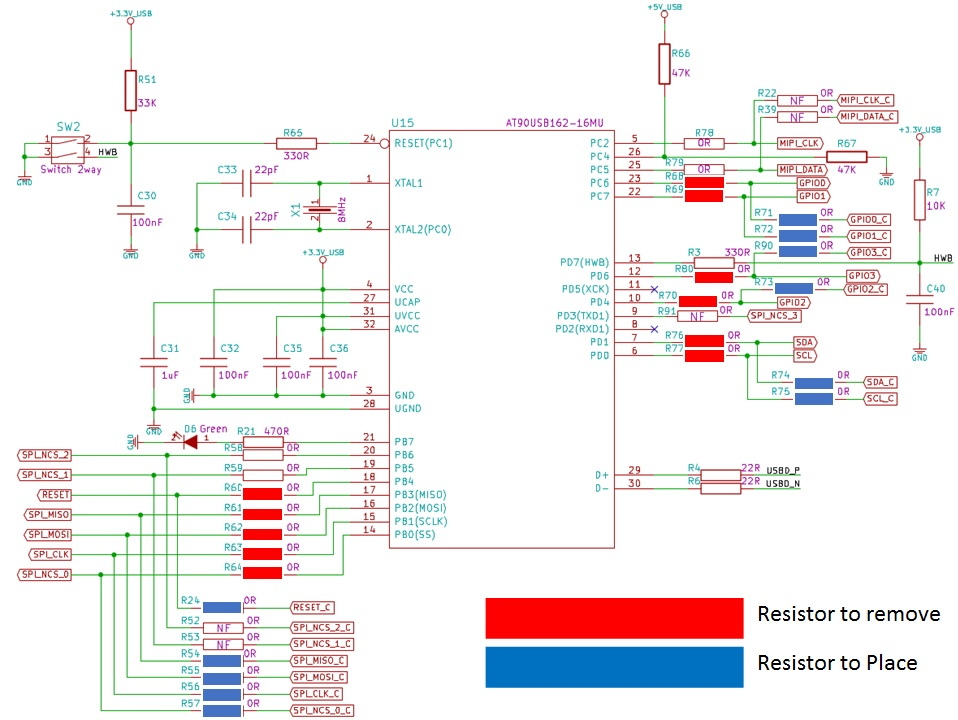
\includegraphics[scale=0.6]{zipper_microcontroller}
		\end{center}
	\end{figure}
	\captionof{figure}{Schematic of Zipper I2C, SPI, and GPIO buses}
	\label{fig:zipper_microcontroller}
	\pagebreak
	\begin{figure}[ht]
		\begin{center}
		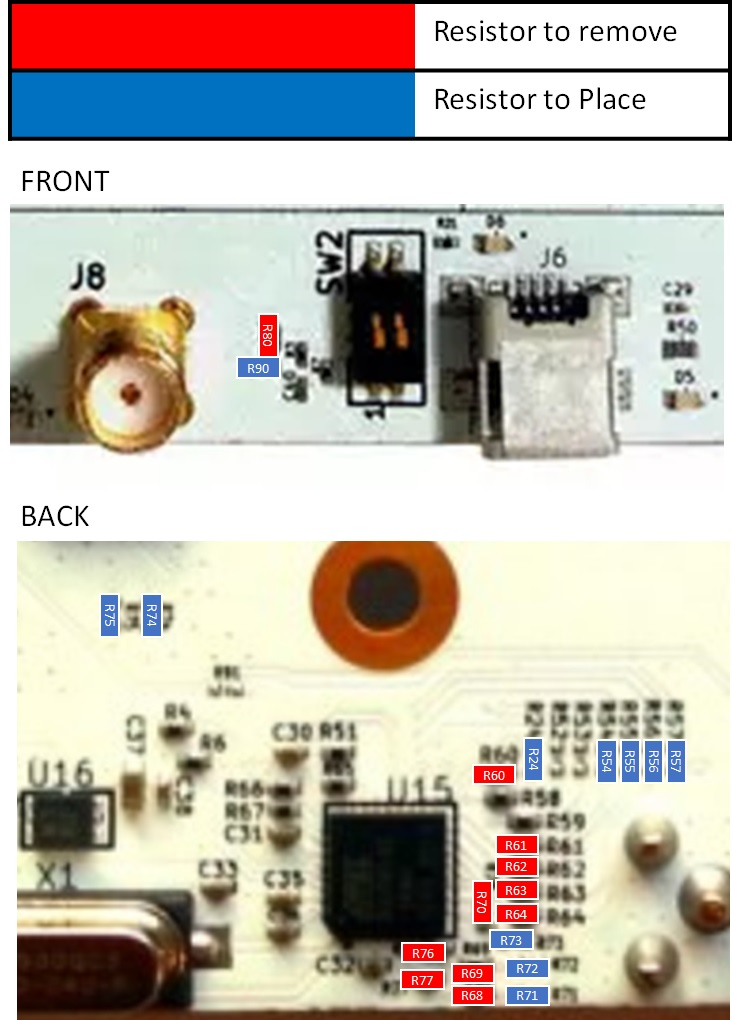
\includegraphics[scale=0.6]{zipper_layout2}
		\end{center}
	\end{figure}
	\captionof{figure}{Layout of Zipper I2C, SPI, and GPIO buses}
	\label{fig:zipper_layout2}
	\pagebreak
\subsection*{Zipper: Add jumper to enable I2C over HSMC}
\normalsize
\textbf{Note: This modification only applies to use with platforms with HSMC connectors (alst4)}\par\medskip
\noindent There is a known layout error in version v1 r1 of the Zipper carrier card which impacts the I2C interface over the HSMC connector. The I2C SDA signal is connected to pin 111 of the HSMC connector, which corresponds to +3.3V on the alst4 (per the HSMC spec). The recommended modification avoids this error, while maintaining support for both FMC and HSMC connections.\par\medskip
\noindent A diagram of the required modifications including instructions can be seen in Figure \ref{fig:zipper_hsmc_i2c}. In summary, a 3 pin header is added to the design to switch between the existing working FMC connection and an unused HSMC pin.
  	\begin{figure}[ht]
	\centering
		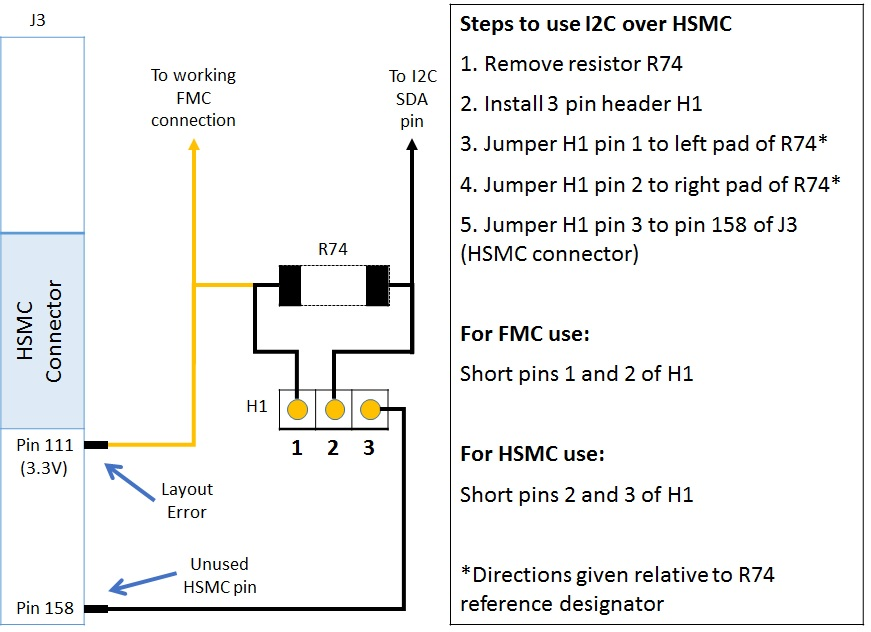
\includegraphics[scale=0.7]{zipper_hsmc_i2c}
		\caption{Diagram and instructions for enabling I2C over HSMC with Zipper carrier card}
	\end{figure}
		\label{fig:zipper_hsmc_i2c}
\subsection*{Connecting the Myriad-RF 1 to the Zipper}
As mentioned above, the Zipper can be connected to platforms via FMC \textit{or} HSMC connectors. Make sure Myriad-RF 1 is connected to the Zipper using the same connection type. So, for example when connecting the Zipper to the alst4 platform via HSMC, make sure the Myriad-RF 1 is connected to the Zipper via HSMC as well.
\pagebreak
  \begin{thebibliography}{1}

  \bibitem{zipper_sch} Zipper v2 r1 Schematic\\
	 Zipper\_v.2\_Schematics\_r.1.pdf (included in this directory)

  \bibitem{dev_kit_manual} Zipper \& Myriad-RF 1 Development Kit Manual\\ https://github.com/myriadrf/reference-development-kit/blob/master/zipper/docs/\\Zipper Development Kit\_1 0r5.pdf

  \bibitem{zipper_layout} Zipper v2 r1 Layout Drawing\\
	 Zipper\_v.2\_Layout\_r.1.pdf (included in this directory)

  \bibitem{myriadrf_sch} Myriad-RF 1 Schematic\\ https://github.com/myriadrf/reference-development-kit/blob/c09ccdbac996ebbbbd2ea3c8fd5f02affb97e6ff/\\rfmodule/v1/VIA\_OFF\_PAD/PDF/MYRIAD\_RF\_Schematics.pdf

  \bibitem{lime_datasheet} Lime Microsystems LMS6002D Datasheet\\
	 http://www.limemicro.com/download/LMS6002Dr2-DataSheet-1.2r0.pdf

  \end{thebibliography}
\end{document}
